%----------------------------------------------------------------------------
\label{LED section}
%----------------------------------------------------------------------------
\input{figures/experiments/redLED/redLED.tex}
%----------------------------------------------------------------------------
%bb defines the bounding box for the pdf
%viewport defines the area of the pdf used
%in sidewaysfigure the last entry in bb moves the caption toward/away the pic
%in sidewaysfigure the second entry in bb moves the pic toward/away the caption
%----------------------------------------------------------------------------
\begin{figure}
\scalebox{0.8}[0.8]{
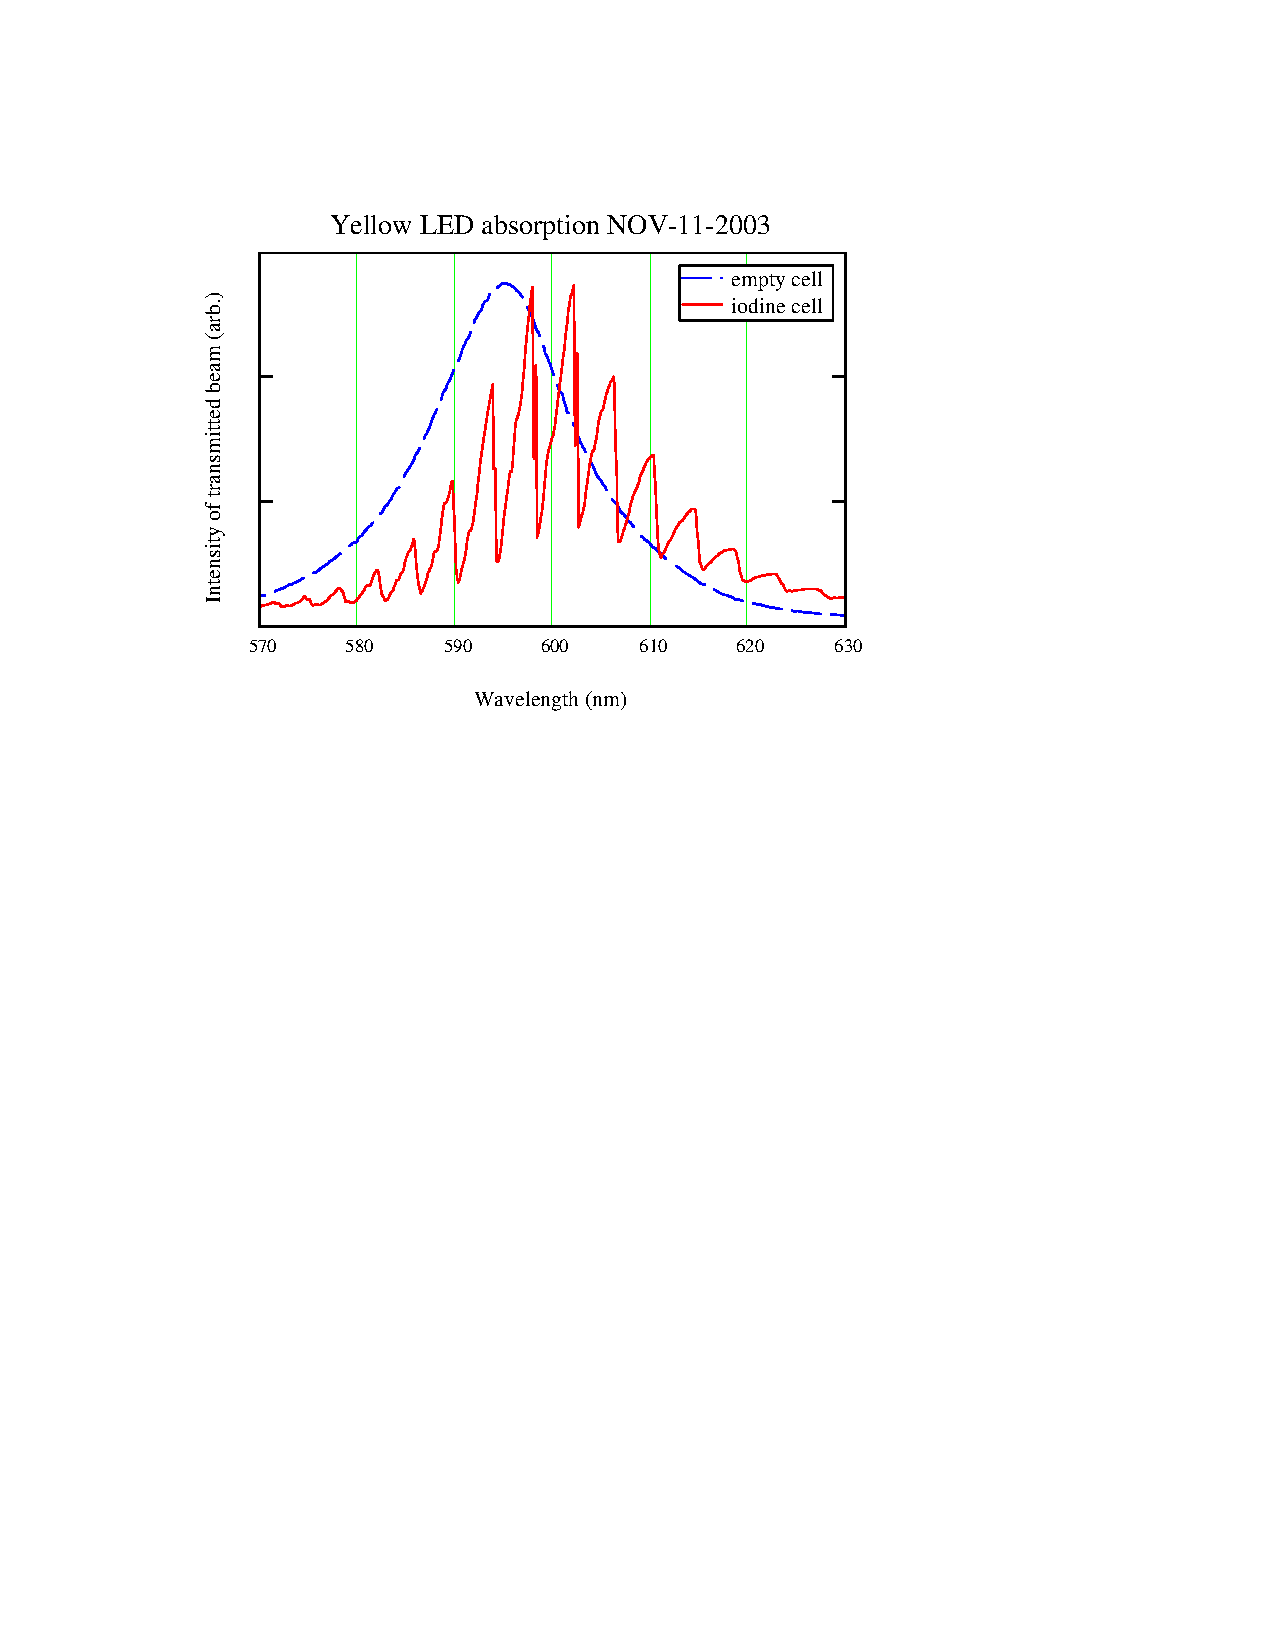
\includegraphics[bb=0 450 489 700]
{yellowLED/yellowLED.pdf}
}
\caption[Yellow LED absorption in molecular iodine]{Yellow LED absorption in molecular iodine. The solid trace is about 5 times smaller than the dashed trace}
\label{yellowLED}
\end{figure}
%----------------------------------------------------------------------------

%----------------------------------------------------------------------------
%bb defines the bounding box for the pdf
%viewport defines the area of the pdf used
%in sidewaysfigure the last entry in bb moves the caption toward/away the pic
%in sidewaysfigure the second entry in bb moves the pic toward/away the caption
%----------------------------------------------------------------------------
\begin{figure}
\scalebox{0.8}[0.8]{
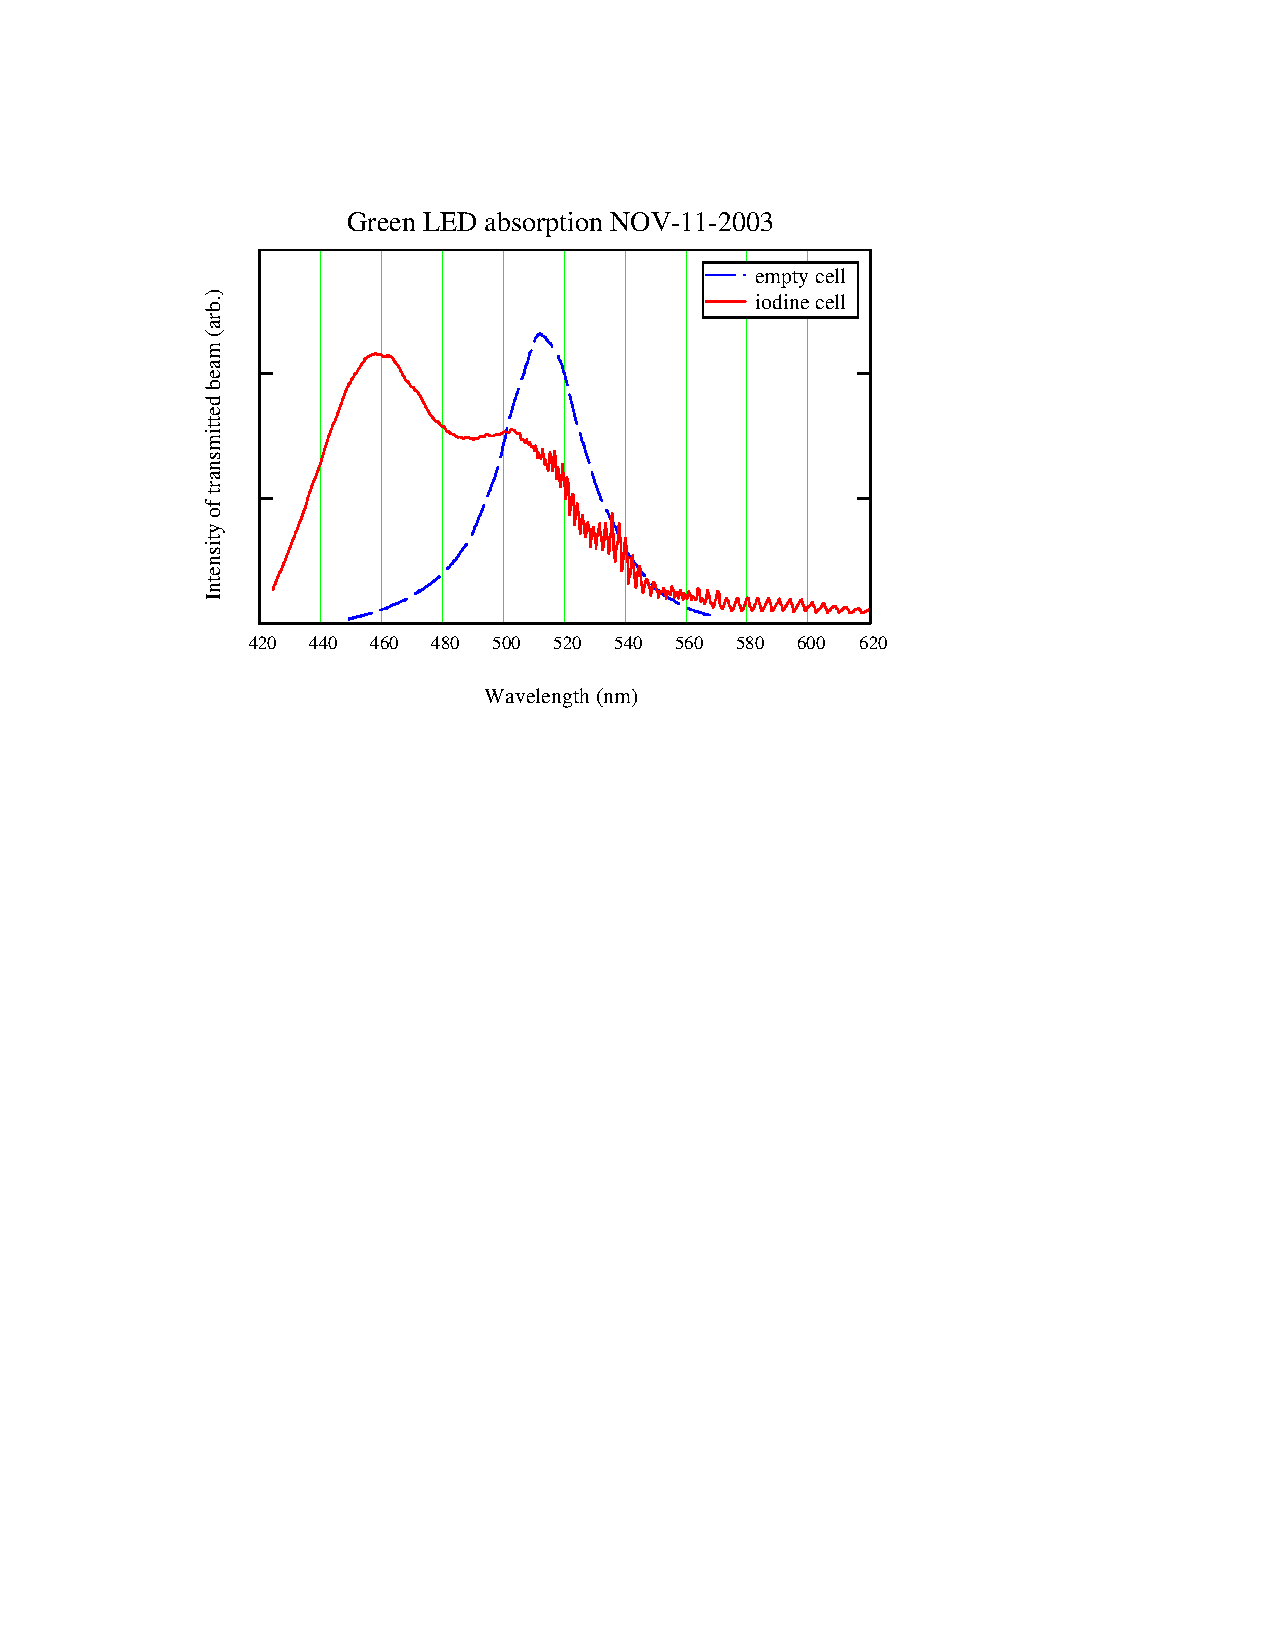
\includegraphics[bb=0 450 489 700]
{greenLED/greenLED.pdf}
}
\caption[Green LED absorption in molecular iodine]{Green LED absorption in molecular iodine. The solid trace is about 10 times smaller than the dashed trace}
\label{greenLED}
\end{figure}
%----------------------------------------------------------------------------

%----------------------------------------------------------------------------
We measure the broadband absorption spectrum of molecular iodine using LED illumination. Three LED's were used: red (see Figure \ref{redLED}), yellow (see Figure \ref{yellowLED}), green (see Figure \ref{greenLED}). The absorption features match those in the literature in shape and spectral position. Also the general observation that iodine exhibits heavier absorption in the green than the red is supported by the data.

As one of the first measurements recorded, these experiments were used to develop the essential components of this spectroscopic study: spectral analysis, light detection, data acquisition, light sources, and sample preparation. A side--view PMT is mounted at the monochromator output and encased in an aluminum foil lined cardboard box; this primitive setup proves very reliable. A chart recorder is used to acquire data; the pen axis is ``linearly'' scanned using a voltage rise from a simple RC circuit. Data processing methods are developed to account for the non-linearity of the voltage rise. Gas lamp calibration procedures are developed for use with the monochromator.

A cell is prepared in a crude fashion by simply loading a sample cell with a few flakes of iodine in an unprotected environment (outdoors, in front of the physics building), closing the cell's greased stop cock, connecting the cell to a mechanical vacuum pump, and evacuating the loaded cell at room temperature. The cell is closed off again, wrapped in heat tape, and temperature stabilized at $150^\circ$ F with a bench top controller and used on the optical bench. Ideally at this temperature the overloaded iodine cell should have a collision lifetime of 11 ns, a density of $1.9\cross10^{17}$ molecules/cm$^3$, and a pressure of 6.8 Torr (from an internal AHI document DN-3300-4 by Dr. Pui K. Lam). The cell is wrapped in aluminum foil giving it a ``baked potato'' appearance -- hereafter, this cell will be referred to as such.

%----------------------------------------------------------------------------
%----------------------------------------------------------------------------
